% 矩形的中点四边形是菱形
\documentclass[tikz,border=4pt]{standalone}
\usepackage{ctex}
\usepackage{amsmath}
\usetikzlibrary{calc}
\begin{document}
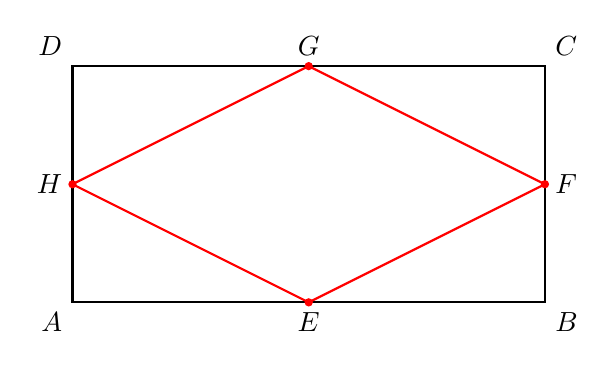
\begin{tikzpicture}[scale=1.0, thick]
  \coordinate (A) at (0, 0);
  \coordinate (B) at (6, 0);
  \coordinate (C) at (6, 3);
  \coordinate (D) at (0, 3);

  \coordinate (E) at ($(A)!0.5!(B)$);
  \coordinate (F) at ($(B)!0.5!(C)$);
  \coordinate (G) at ($(C)!0.5!(D)$);
  \coordinate (H) at ($(D)!0.5!(A)$);

  \draw (A) -- (B) -- (C) -- (D) -- cycle;
  \draw[red, thick] (E) -- (F) -- (G) -- (H) -- cycle;
  \foreach \p in {E,F,G,H} \fill[red] (\p) circle (1.5pt);

  \node[below left]  at (A) {$A$};
  \node[below right] at (B) {$B$};
  \node[above right] at (C) {$C$};
  \node[above left]  at (D) {$D$};
  \node[below] at (E) {$E$};
  \node[right] at (F) {$F$};
  \node[above] at (G) {$G$};
  \node[left]  at (H) {$H$};
\end{tikzpicture}
\end{document}
